\subsection{Web Testing}
There are three components to test in the web system. The first is the API endpoints and backend functionality. The second is the integration of the user interface and the API. And lastly, the functionality of the socket server must be tested as well.
\subsubsection{API Testing} \label{sec:api-test}
There will be two key ways that the API testing will be conducted: unit tests and integration tests. In a web context these are slightly different than in a strict engineering context. Generally speaking, a unit test of a an API or backend service checks that business logic is working as expected. For example, in our project there will be some filter to grab the correct information from the database based on the plant bed. In a unit test, we might mock the database with dummy data and ensure that this is occurring properly.

On the other hand, the integration test of the API will be done in two ways which will also serve to self-document the API. Using a mock client, we can program requests for certain conditions such as certain failure or success. In this instance, the request is actually routed through all the middleware, connects to the database and performs the function. We can validate the result by looking at the database and ``asserting'' all these values are correct.

The self-documenting test will be done using Swagger and OpenAPI 3.0. Swagger is a tool for building UI elements that can build and run requests on the web server and the response elements can be validated against data types. See \autoref{fig:swagger} for a visual representation as to what this might look like.

\begin{figure}[H]
    \caption{Swagger UI example}
    \label{fig:swagger}
    \centering
    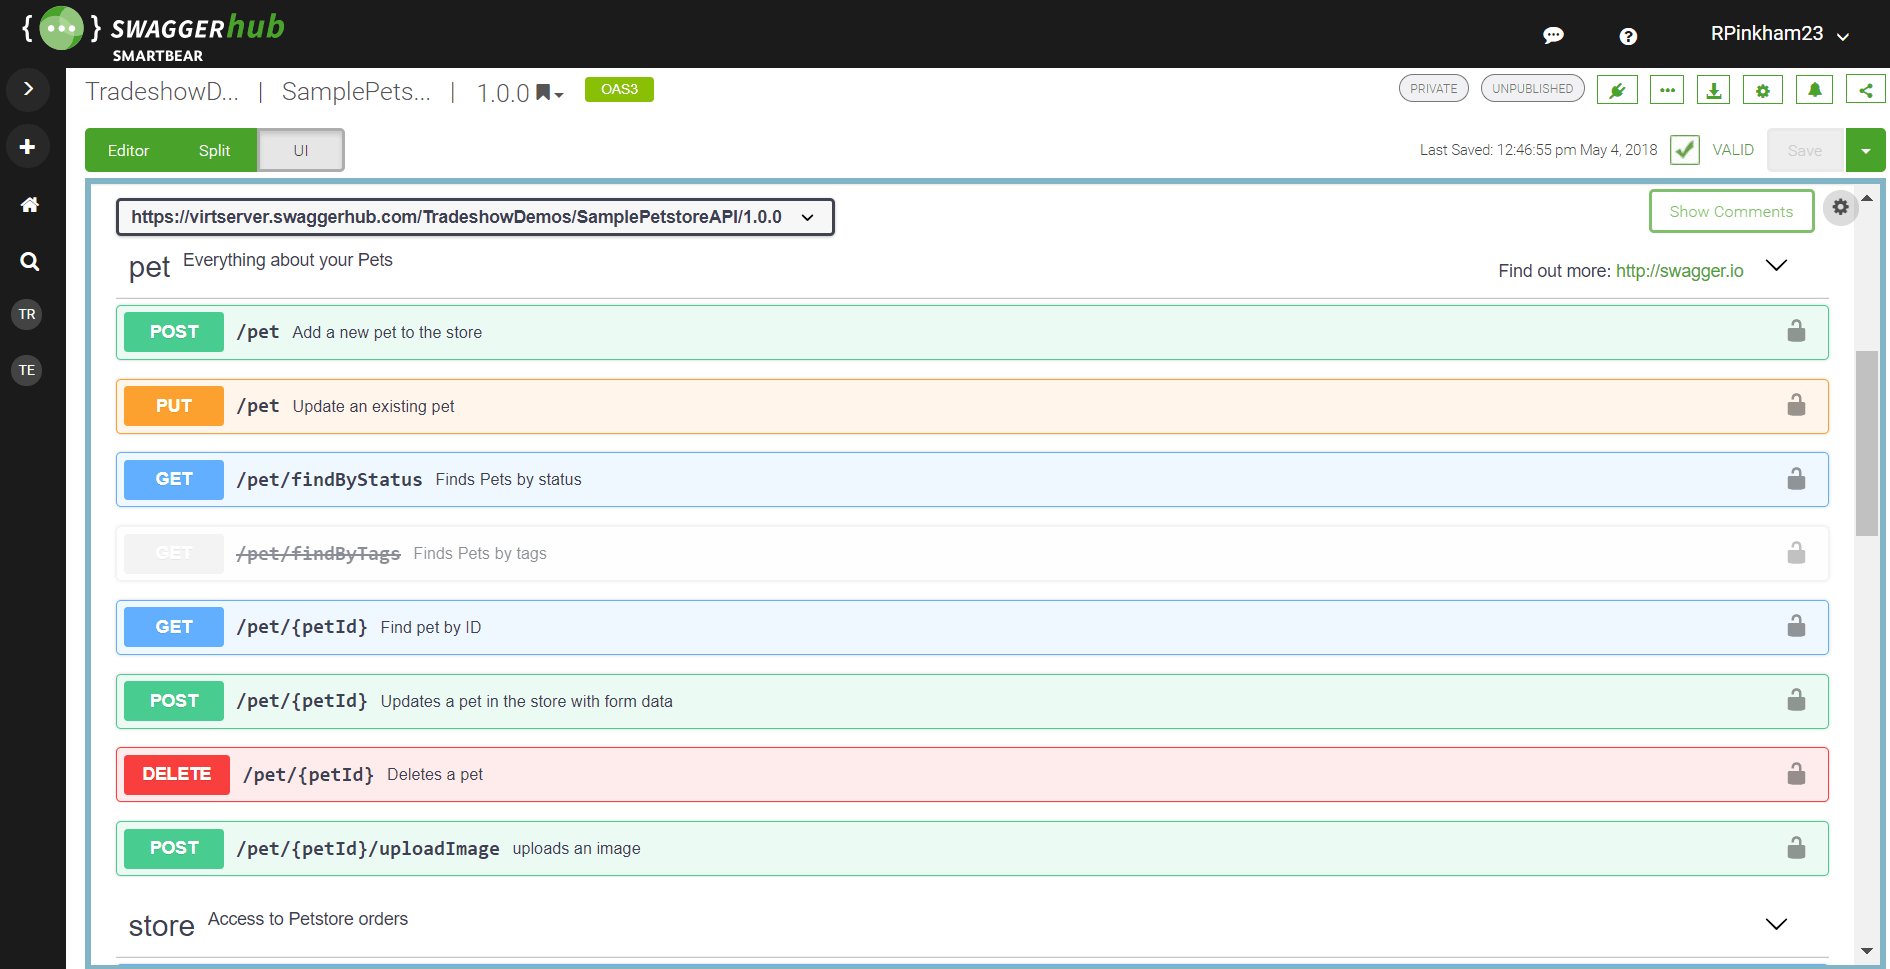
\includegraphics[width=\textwidth]{images/Swagger.png}
\end{figure}

\paragraph{Test Plan}
The unit tests and integration tests will be ran on each push of code changes to GitHub and through the use of GitHub actions, passing tests can be validated and added to the branch protection rules. Branch protection rules prevent broken code from becoming a part of the code base. These rules are integral to our test plan. See \autoref{fig:github-actions} to see how passing/failing tests would appear.

\begin{figure}[H]
    \caption{GitHub workflow}
    \label{fig:github-actions}
    \centering
    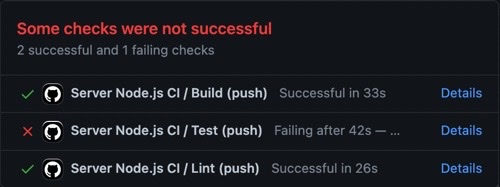
\includegraphics[width=\textwidth]{images/github.jpeg}
\end{figure}

The key to integrating this quality of life feature is designing good tests. The API in general has four functions: create, read, update, delete. The unit tests will be configured to ensure error handling and data composition are done properly. For example, when making a request about a particular plant bed, if the ID does not exist, we want to the error to be verbose but the request to fail. Similarly, we want to ensure that the logic for building data tables from the database occurs properly. The integration tests will have one well-formed request and one malformed request in order to test the error handling and full integration of correct data.

\subsubsection{User Interface Testing}
There are two key ways to be able test the user interface: using prototypes and integrating with the backend. Using React the expectation is that the user interface will be reactive. Thus, we use prototypes which are components built on hardcoded data that reacts to user input, thus we can test the viability of components. For example, we want to test that a graph component when hovered shows the data point in a floating box. We would build the UI with static data and ensure this result in the UI. Secondly, we need to test that the integration with the backend is working properly. This occurs by running an ``end-to-end'' test. Essentially, this is a final test. The plan is to give the testable product to consumers and let them have their way with the UI to discover bugs.

React comes packaged with a testing library that allows for quick unit testing of components in a similar way to the unit tests mentioned in the API section (\ref{sec:api-test}). Implementing this will automate the unit tests as opposed to manually building the entire program and checking manually each component. We will be using \href{https://testing-library.com/docs/react-testing-library}{this documentation} to build out the automatic test suite.

\subsubsection{Socket Testing}
Unit testing sockets will be done in a similar way to unit testing the API endpoints however the unit test will create a mock socket client and the two features will be tested separately: sending and receiving.

\paragraph{Sending Packets to Client}
To test that the client is receiving the packets properly in isolation, the mock client will open a connection to the server and the unit test will call the send packet function. The client will then expect certain values in a certain character set and this will all be validated by the assertion.
\paragraph{Receiving Packets from Client}
The mock client will send a packet to the socket server with static data that is formatted exactly as it would come from the MCU. From there, the unit test will assert that the received packet has all the required metadata, uses the correct character set and is formatted properly.